\documentclass[8pt]{beamer}

\usetheme{Singapore}

%Russian-specific stuff
\usepackage[T2A]{fontenc}
\usepackage[utf8]{inputenc}

\usepackage{hyphenat}
\hyphenation{ма-те-ма-ти-ка}
%end of Russian-specific packages

\usepackage{graphicx}
%\usepackage{subfigure}
\usepackage[labelformat=empty]{caption}
\usepackage[labelformat=empty]{subcaption}

\usepackage{wasysym}

\title{Микроквазары}
\subtitle{МФК `Космические тайны рентгеновского неба'}
\titlegraphic{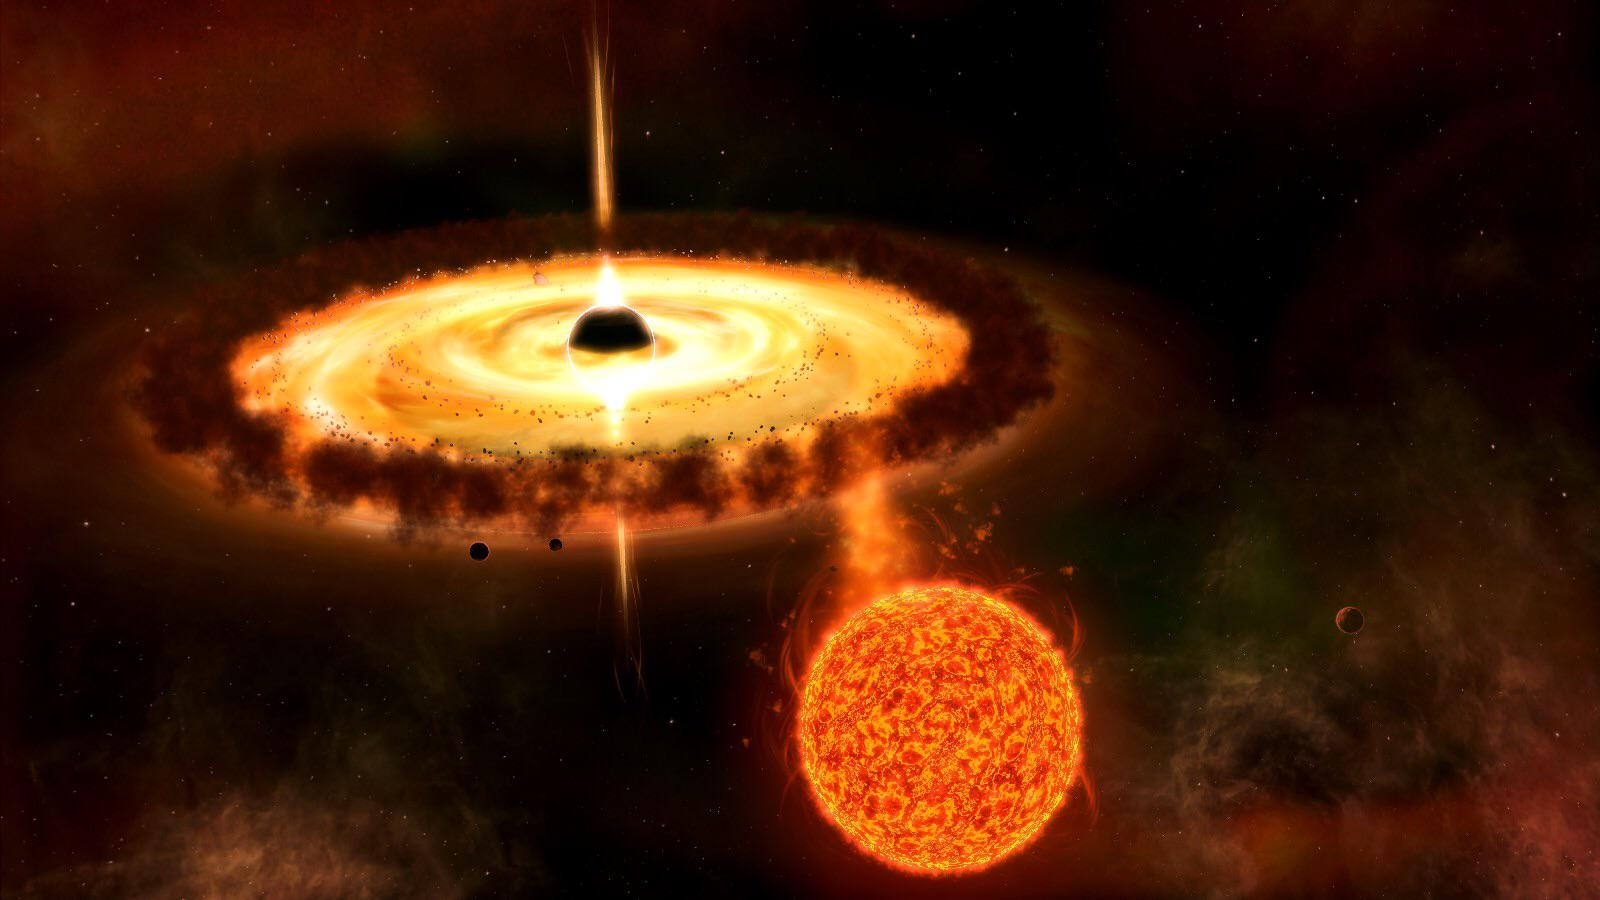
\includegraphics[width=.6\textwidth]{resources/microquasar-stellaris.jpg}}
\author{Фельдшеров Сергей}
\date{20 Апреля 2022}
%\date{}

\begin{document}

%\maketitle

\begin{frame}
	\titlepage
\end{frame}

\section{Введение}

\begin{frame}
	\frametitle{Ярчайшие объекты во вселенной}
	Активные ядра галактик - объекты с мощным электромагнитным излучением, состоящие из:
	\begin{itemize}
		\item сверхмассивной чёрной дыры
		\item окружающего её аккреционного диска
	\end{itemize}\pause
	Электромагнитное излучение исходит от разогретого трением вещества аккреционного диска.
	\begin{figure}[h]
	    \centering
		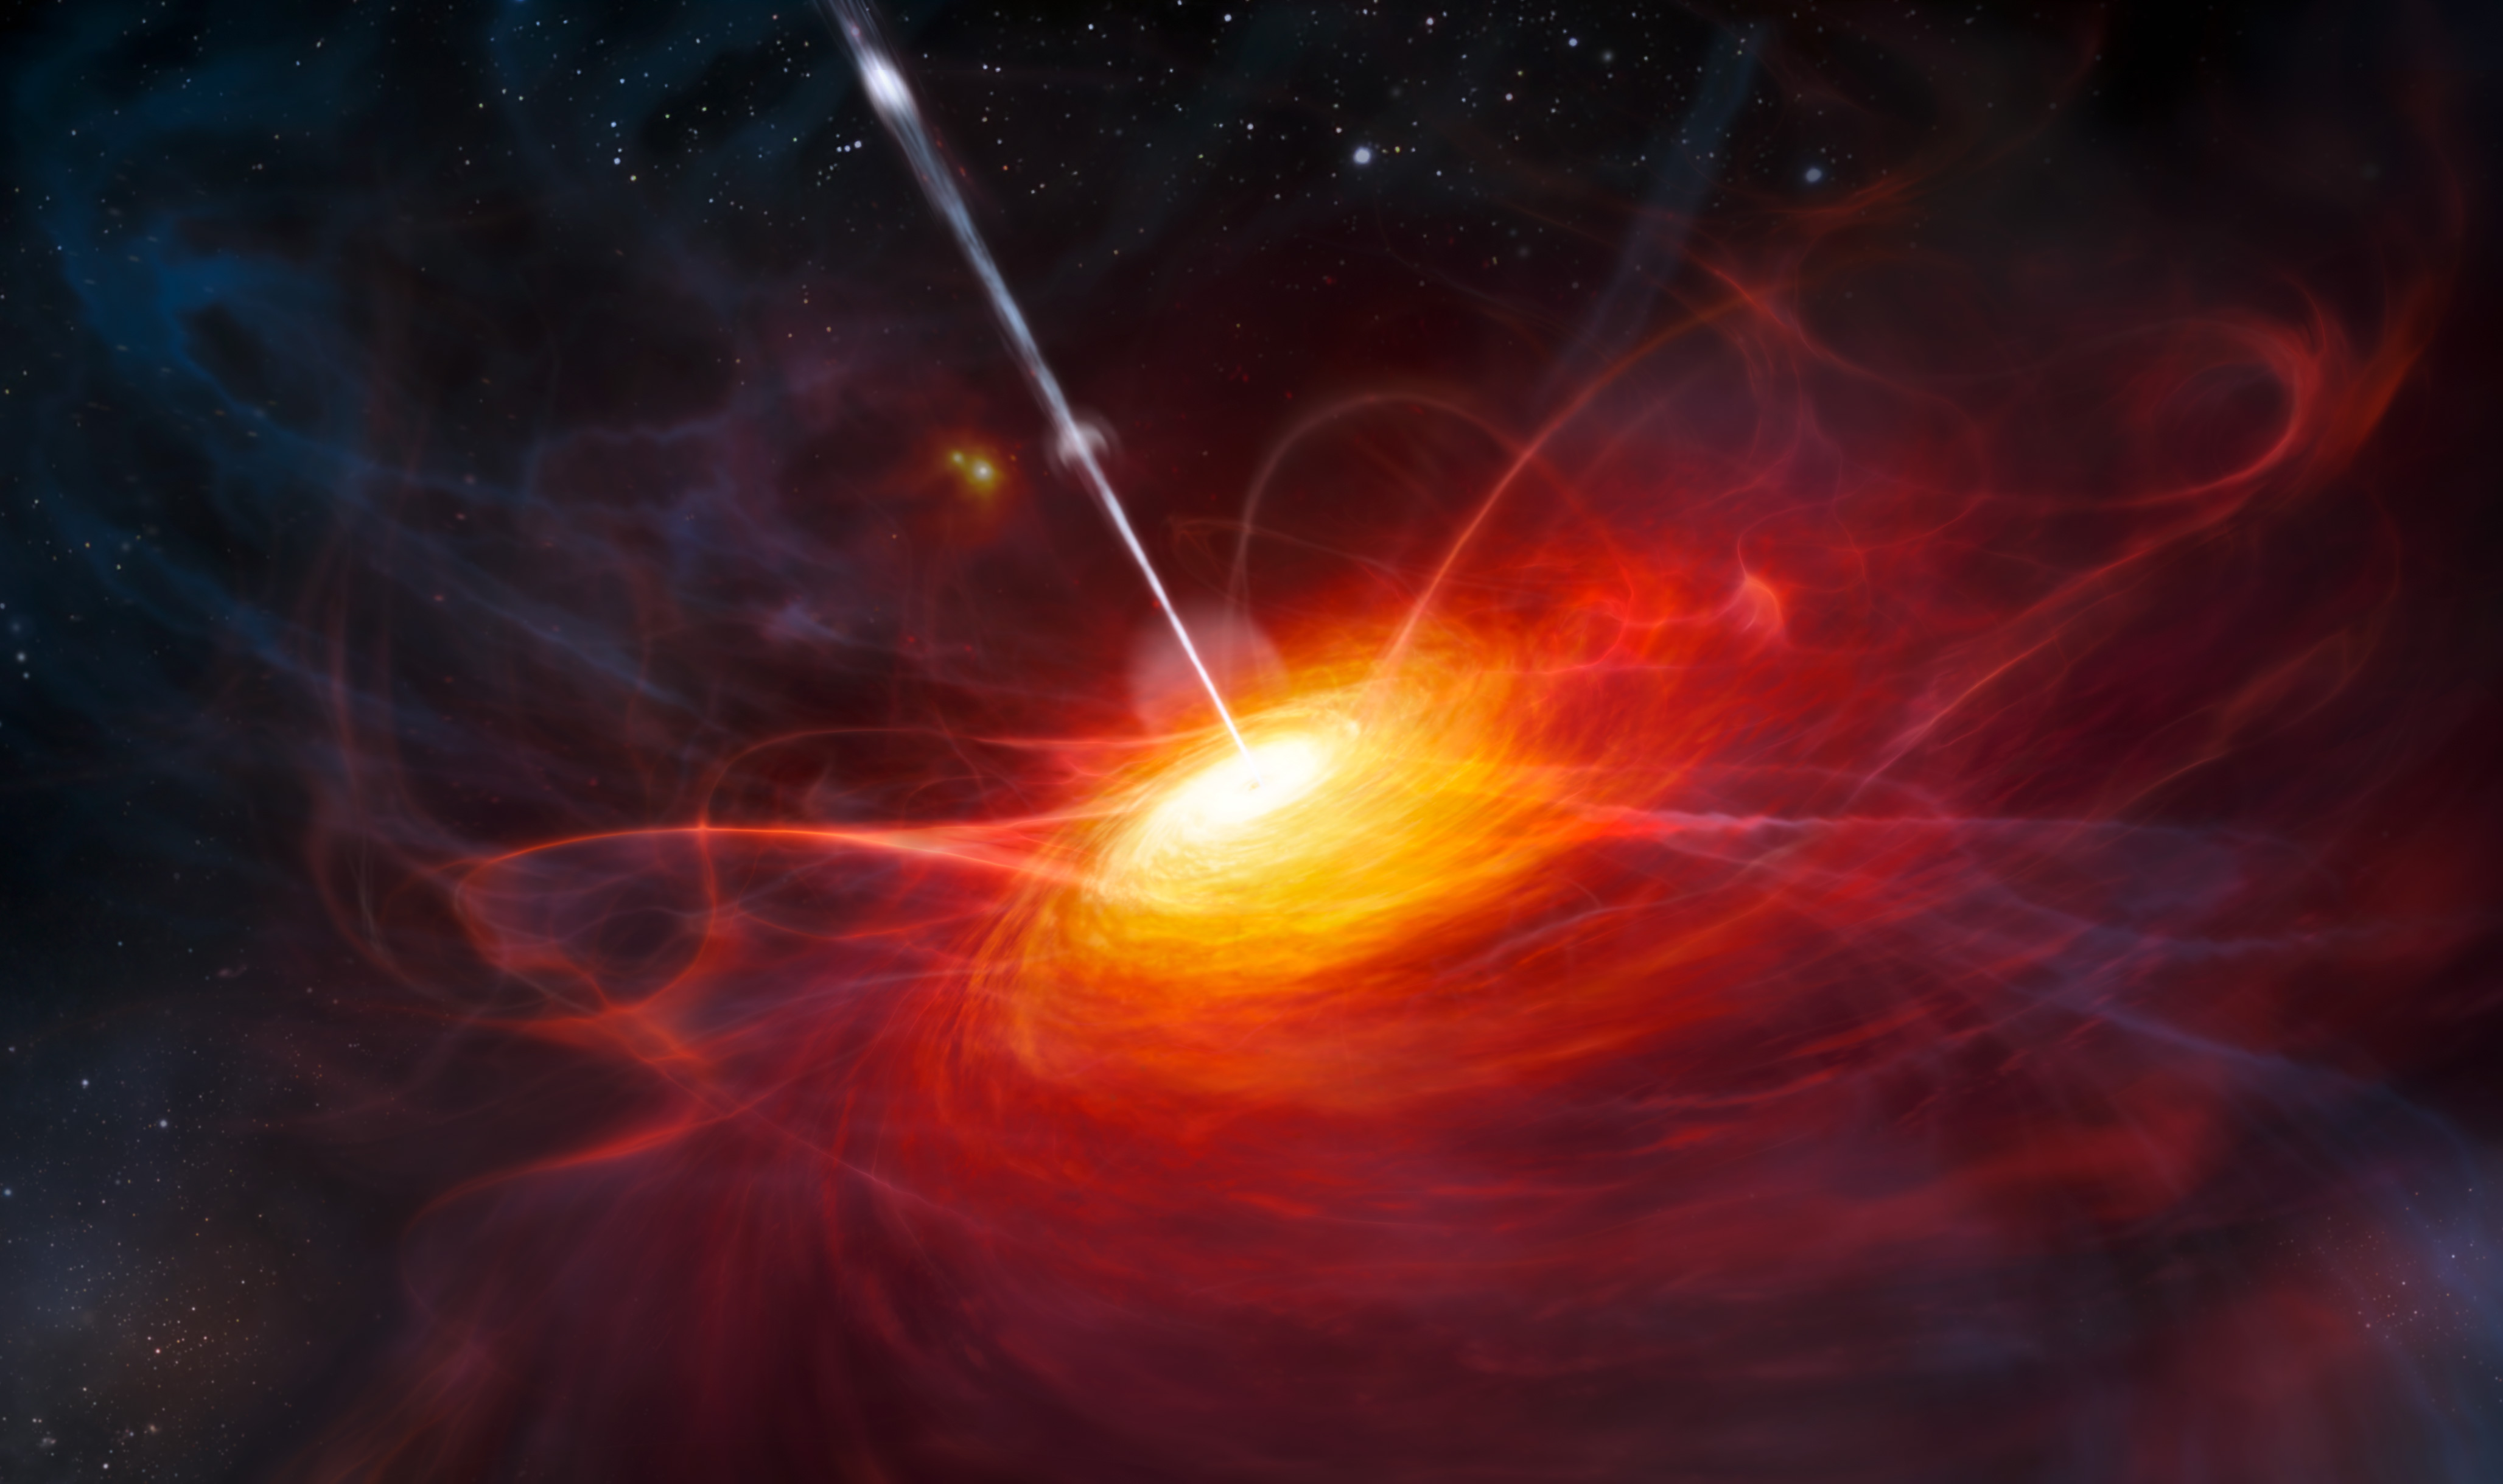
\includegraphics[width=.5\textwidth]{resources/quasar-rendering.jpg}
		\caption{Аккреционный диск квазара ULAS J1120+0641, обнаруженного в 2011 году, в представлении художника.}
	\end{figure}
	Объекты, определяемые в эту группу: радиогалактики, Сейфертовские галактики, квазары.

\end{frame}

\begin{frame}{Микроквазары}
    Микроквазарами называют двойные звёздные системы с похожим принципом `подпитки' энергией. Они состоят из компактного объекта, перетягивающего на себя веществом звезды-компаньона.
    \begin{figure}
        \begin{subfigure}{0.45\textwidth}
            \centering
            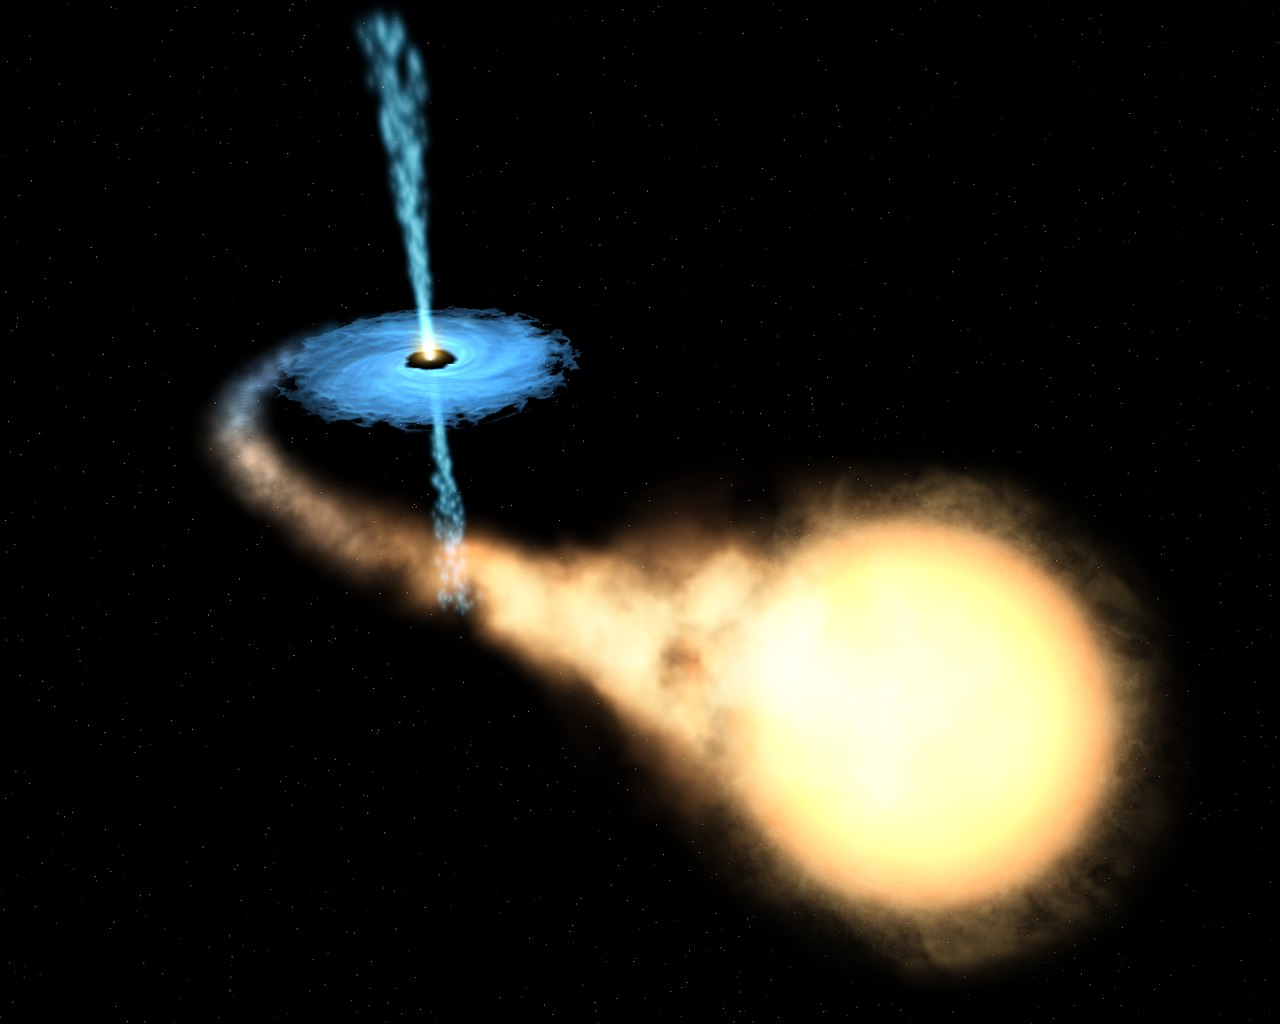
\includegraphics[width=\textwidth]{resources/accretion-disk-illustration.jpg}
            \caption{микроквазар в представлении художника}
        \end{subfigure}
        \begin{subfigure}{0.45\textwidth}
            \centering
            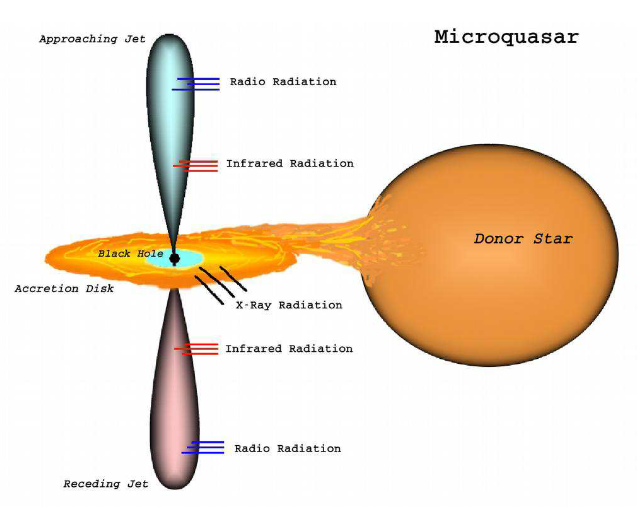
\includegraphics[width=\textwidth]{resources/microquasar-scheme.png}
            \caption{схема микроквазара}
        \end{subfigure}
    \end{figure}
\end{frame}

\begin{frame}{Активные ядра галактик vs микроквазары}
    Энергия АЯГ появляется благодаря сверхмассивной чёрной дыре ($\geq 10^6 M\astrosun$). Рентгеновские двойные системы формируются обычной звездой и `выроджденным' объектом (нейтронной звездой или чёрной дырой в несколько солнечных масс).
    \begin{figure}
        \centering
        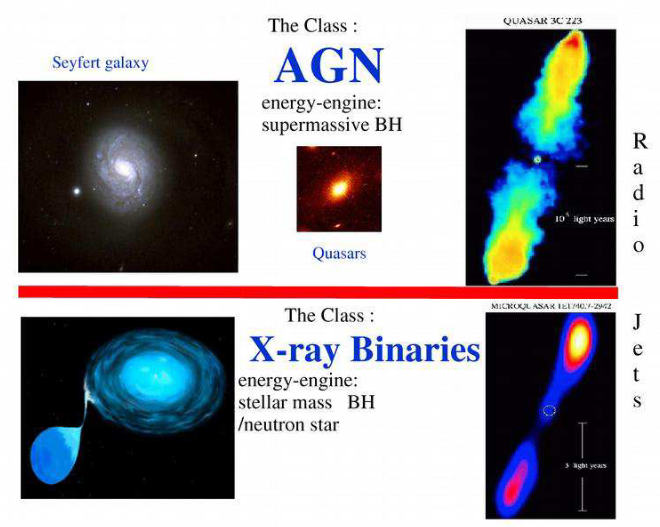
\includegraphics[width=0.7\textwidth]{resources/agn-vs-xray-binaries.png}
    \end{figure}
\end{frame}

\begin{frame}
	\frametitle{Некоторые известные микроквазары: SS 433}
	В 1979 году был открыт необычный объект, излучавший в рентгене и радиодиапазоне:
	\begin{figure}[h]
		\begin{subfigure}{0.45\textwidth}
		    \centering
			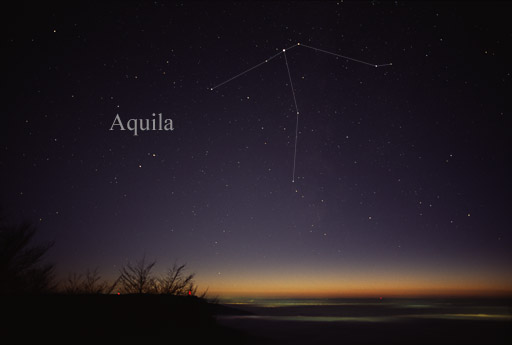
\includegraphics[height=.5\linewidth]{resources/AquilaCC.jpg}
			\caption{Созвездие Орёл}
		\end{subfigure}
		\begin{subfigure}{0.45\textwidth}
		    \centering
			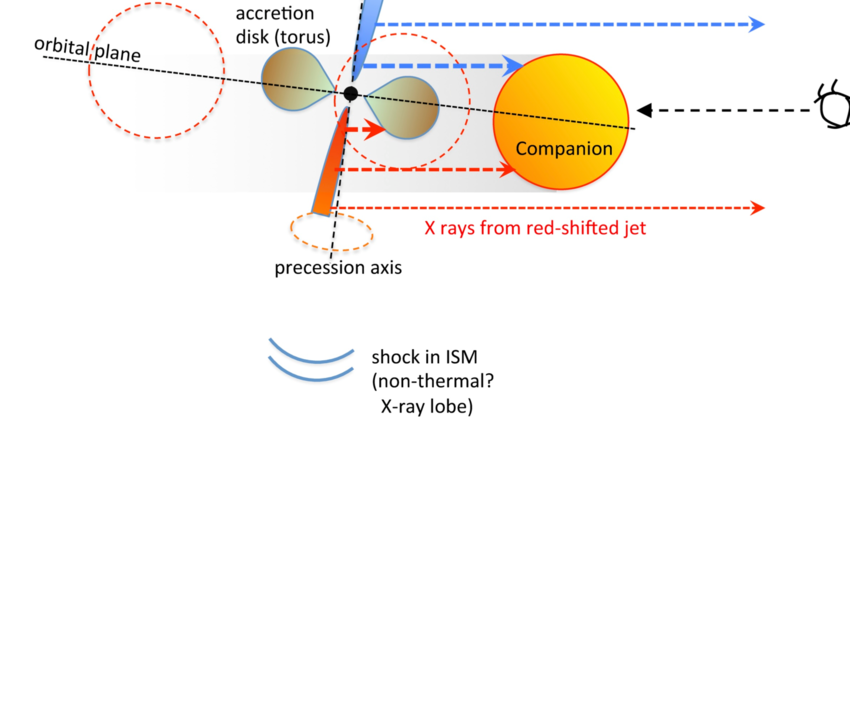
\includegraphics[height=.5\linewidth]{resources/ss-433-schematic-view.png}
			\caption{Схематическое изображение SS 433, Hirofumi Noda}
		\end{subfigure}

		%\caption{Объект SS 433}
	\end{figure}

\end{frame}

\begin{frame}{Некоторые известные микроквазары: GRS 1915+105}
    \begin{figure}
        \begin{subfigure}{0.45\textwidth}
            \centering
            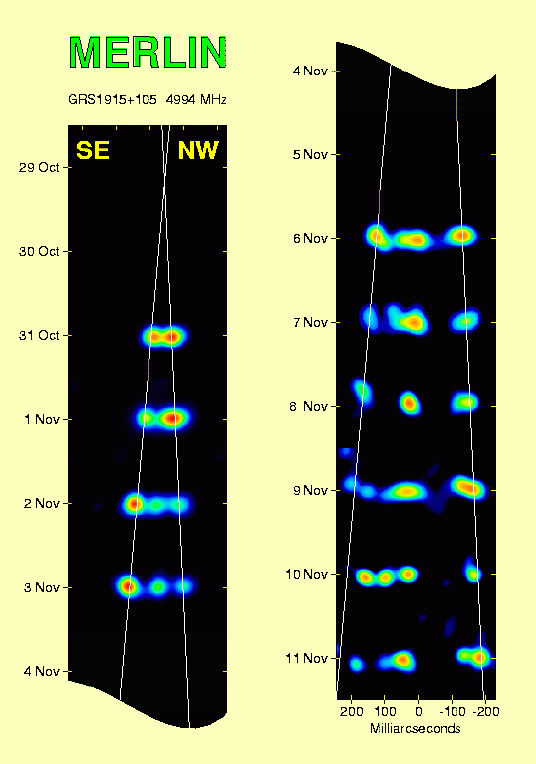
\includegraphics[height=.9\linewidth]{resources/Merlin-GRS1915.png}
            \caption{Радиотелескопы MERLIN}
        \end{subfigure}
        \begin{subfigure}{0.45\textwidth}
            \centering
            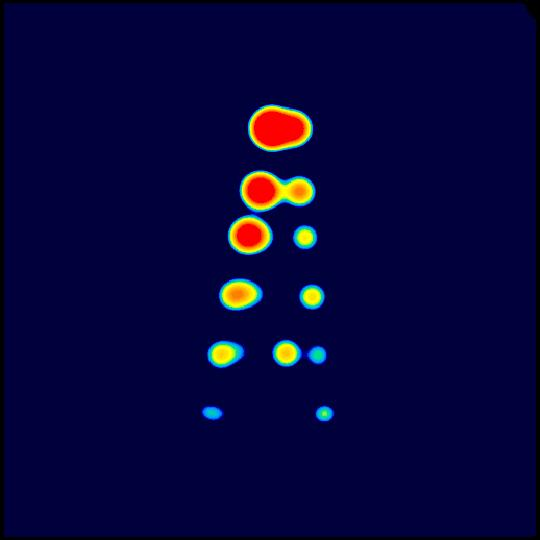
\includegraphics[height=.9\linewidth]{resources/Grs1915_radio.jpg}
            \caption{Радиотелескопы VLA}
        \end{subfigure}
        
        \caption{Наложенные последовательности изображений, сделанных в течение нескольких дней и в течение месяца}
    \end{figure}
\end{frame}

\section{Процессы аккреции и выброса материи}

\begin{frame}{Что известно об образовании микроквазаров}
    Механизмы, объясняющие присутствие компактного объекта в двойной системе, зависят от массы
    компаньона:
    \begin{enumerate}
        \item звезда малой массы: формирование нейтронной звезды/компактного объекта предшествовало появлению двойной системы
        \item тяжёлая ($\geq 5M\astrosun$) звезда: масштабный перенос массы до взрыва сверхновой
    \end{enumerate}
    \centering
    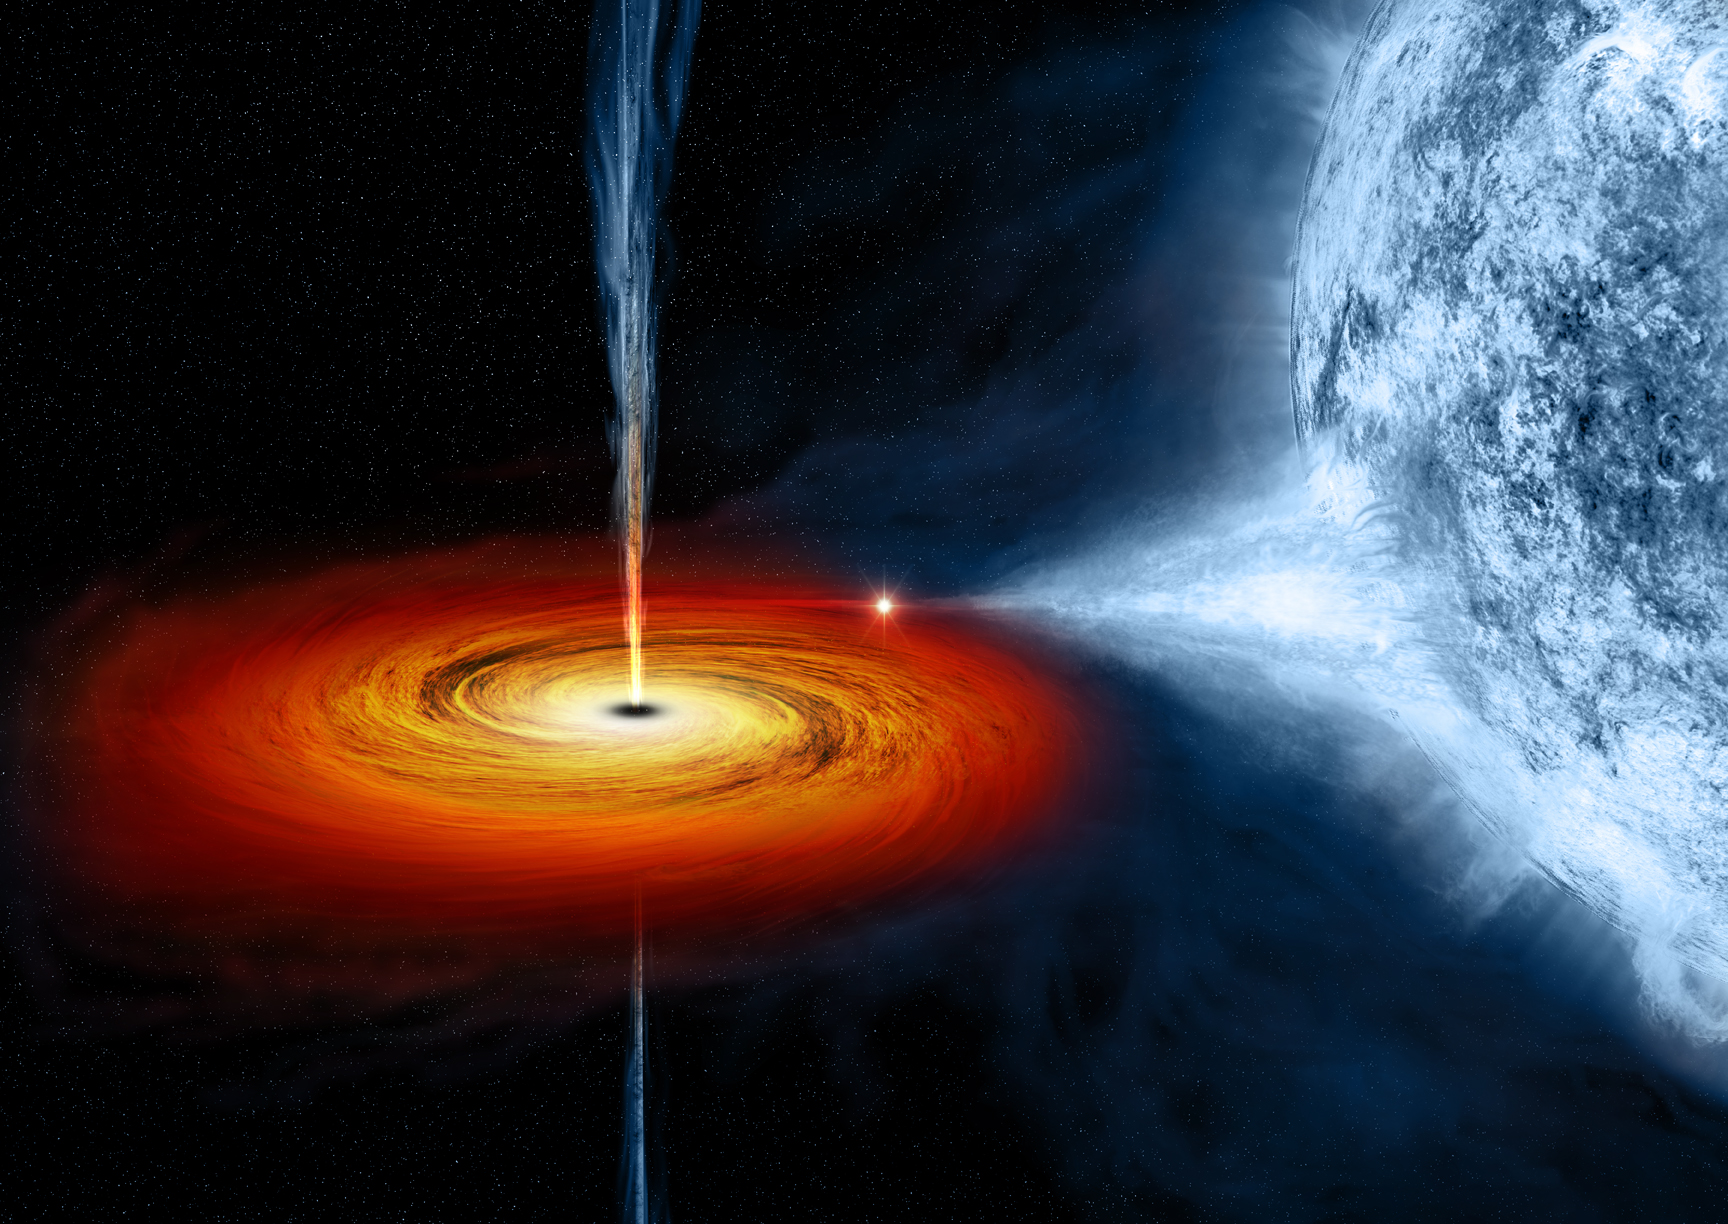
\includegraphics[width=0.6\textwidth]{resources/accretion-illustration.jpg}
\end{frame}

\begin{frame}{Аккреция и перенос энергии}
    Перенос материи сопровождается двумя процессами:
    \begin{itemize}
        \item Благодаря силам вязкости угловой момент аккрецируемой материи перераспределяется,
            и кольцо становится диском.\pause
        \item Происходит рассеивание тепла, возникающего из-за `трения'.\pause
    \end{itemize}
    Температура достигает максимума на орбите с наибольшей скоростью:
    \[
        T_{in} \simeq 2 \cdot 10^7 \left(\frac{M_X}{M_{\astrosun}}\right)^{-1/4} K,
    \]
    что и даёт Рентгеновское излучение бинарных систем с компактным объектом околозвёздной массы.
    
    Однако, существует ограничение на то, какое количество энергии высвобождается при аккреции.
    Это связано с тем, что давление излучения может превысить гравитацию компактного объекта.
\end{frame}

\begin{frame}{Высвобождение джетов: формирование магнитной спирали}
    Наличие небольшого вертикального магнитного поля приводит его `наматыванию'.\pause
    \begin{figure}
        \centering
        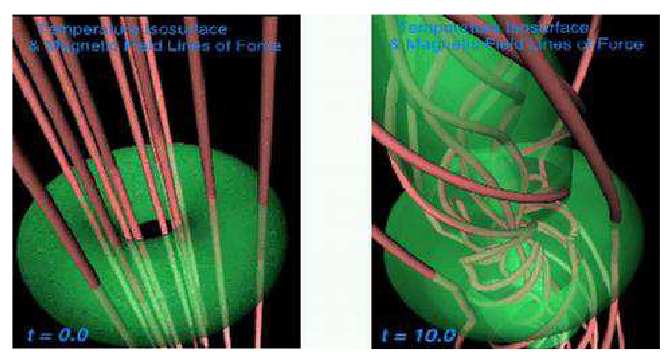
\includegraphics[width=\textwidth]{resources/magnetic-winding.png}
    \end{figure}
\end{frame}

\begin{frame}{Высвобождение джетов: ветер}
    Падение энергии диска аккреции ведёт к лавинообразному падению материи на компактный объект.
    Падающая материя `утягивает' за собой магнитное поле, и может произойти его замыкание, что
    приводит к прерыванию джетов.
    \begin{figure}
        \centering
        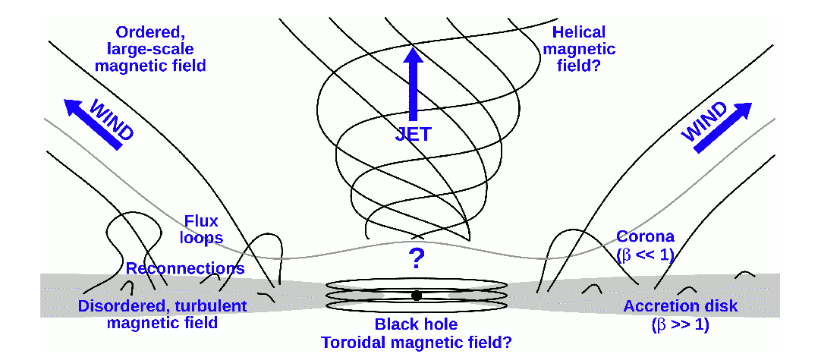
\includegraphics[width=\textwidth]{resources/jet-accretion-interaction.png}
    \end{figure}
    
\end{frame}

\begin{frame}{Сильные магнитные поля и рентгеновские пульсары}
    Наличие сильного магнитного поля предотвращает формирование джетов. Однако, аккрецирующие нейтронные звёзды с сильным магнитным полем также излучают в рентгеновском диапазоне.
    \begin{figure}
        \centering
        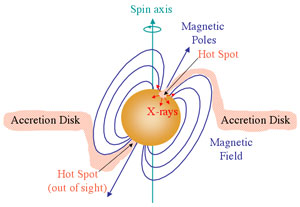
\includegraphics[height=.4\textwidth]{resources/x-raypulsar.jpg}
    \end{figure}
\end{frame}

%\section{Наблюдения}
%
%\begin{frame}
%	\frametitle{Как это выглядит (в рентгеновском диапазоне)?}
%	Тут должно быть про то, как микроквазары излучают. Вообще надо слайд про оптику тоже, и про гамма и радио.
%\end{frame}

%https://arxiv.org/pdf/astro-ph/0506731.pdf



\end{document}
